\part{Theoretische Grundlagen}
\label{sec:theory}

\section{Technische Voraussetzungen}
Im Rahmen dieser Bachelorarbeit werden verschiedenste Technologien verwendet und auf ihnen aufbauende Werkzeuge zu Hilfe genommen. Um zu verstehen, wo Probleme lokalisiert sind und wie solche Schwachstellen zu finden sind, muss man sich mit dem vorhandenem Technologiestack auseinandersetzen und ihn analysieren.
\begin{description}
  \item[Server] Ein Server ist ein Computer, der Informationen und Dienste für andere Computer zur Verfügung stellt.
  \item[Betriebssystem] Die Software, die auf dem Server läuft. In der pludoni GmbH wird das Linux-Derivat Debian eingesetzt.
  \item[Datenbank] Als Datenbank wird eine strukturierte Sammlung von Daten bezeichnet. Einer der häufigsten Vertreter, gerade im Zusammenhang mit PHP-Webanwendungen, ist MySQL.
  \item[Web Server] Der Web Server ist für die zuverlässige Auslieferung von Webseiten zuständig. Er beantwortet die Anfragen, die die Nutzer mit Hilfe des Browsers stellen. In der pludoni GmbH wird f\"ur diesen Zweck Apache eingesetzt.
  \item[PHP] ist eine dynamische, typisierte Skriptsprache. Sie ist speziell f\"ur die Webprogrammierung geeignet, da sie direkt in HTML eingebettet werden kann.\citep{PHP2011} In PHP kann prozedural und objektorientiert programmiert werden. Besonders gut unterst\"utzt werden alle Arten von Datenbanken. Durch die gro\ss{}e Entwicklergemeinde gibt es viele Erweiterungen f\"ur PHP. So kann Dank PHP auch sehr leicht mit anderen Services kommuniziert werden, beispielsweise IMAP f\"ur die E-Mail-Server Kommunikation.\citep{PHP2011a}
  \item[Drupal] ist ein CMS und Framework, welches in PHP geschrieben ist und viele direkt nutzbare Funktionen mitbringt. Dazu gehören unter anderem Administrationsoberflächen, News-Aggregatoren, Veröffentlichungsabläufe für Artikel und Blogbeiträge sowie Suchmaschinenoptimierungen. Außerdem ermöglicht Drupal die Installation weiterer, durch Nutzer entwickelte, Module. Dadurch wird eine fast unbegrenzte Funktionsvielfalt ermöglicht. Im vorliegenden Fall wird Drupal in der Version 5 eingesetzt.
  \item[Client] Der Browser des Nutzers erwartet in der Regel ein HTML Dokument. Dies wird durch Drupal generiert und vom Webserver ausgeliefert. Dabei werden Bilder verarbeitet, JavaScript Skripte ausgeführt und andere Elemente, wie Flash-Applikationen und Videos, berechnet. 
\end{description}
In Abbildung \ref{fig:techstack} ist eine schematische Darstellung eines Webseitenaufrufs skizziert. Die orangenen Pfeile stellen eine Anfrage da und die gr\"unen Pfeile die Antworten.
\begin{figure}[!ht]
  \centering
  \includegraphics[scale=1.0]{material/techstack.png}
  \caption{Grunds\"atzlicher Ablauf eines Webseitenaufrufs.}
  \label{fig:techstack}
\end{figure}

\section{Methoden der Web-Performance-Optimierung}
Die Methoden zur Leistungssteigerung können wie im Technologiestack untergliedert und jedes Element kann für sich betrachtet werden.

\begin{description}
  \item[Serverhardware] Der einzige Parameter, der am Server verbessert werden kann, ist seine Leistung, dass heißt Datendurchsatz und Rechengeschwindigkeit. Dies geschieht durch CPU Upgrades oder Arbeitsspeichererweiterung. Weitergehend kann man die Festplattenzugriffsgeschwindigkeiten durch RAID-Verbünde und neue Technologien wie SSD-Speicher verbessern. Wenn ein einzelner Server nicht ausreicht, k\"onnen auch zus\"atzliche Server zur Lastverteilung genutzt werden. Entweder es werden die verschiedenen Dienste, die der Server normalerweise anbietet, auf mehrere Server verteilt oder es wird der Server repliziert und die Last auf alle Server gleichm\"a\ss{}ig verteilt.
  \item[Betriebssystem] Der Ansatzpunkt für Verbesserungen auf Betriebssystemebene ist Memory-Mapping, dass heißt Speicherbereiche, die normalerweise auf der Festplatte liegen, werden in den Arbeitsspeicher umgelagert, um die Latenzen zu verringern. Dies wird genutzt, um Caches zu beschleunigen, die normalerweise von der Festplatte lesen.
  \item[Datenbank] Auf Datenbankebene kann im Fall von MySQL nur beschränkt optimiert werden. Zum einen sind bei häufig genutzten Tabellen Indizes anzulegen und zum anderen kann man MyISAM statt InnoDB nutzen, um performanter zu sein. Datenbanken k\"onnen auf einem eigenen Server betrieben werden. Falls sie sehr hohen Belastungen ausgesetzt werden, k\"onnen durch Replikation mehrere Server die Datenbanklast tragen.
  \item[Web Server] Optimierungen am Webserver sind sehr schwierig, da die Webserver-Performance hauptsächlich von der Serverleistung abhängt. Die Anzahl der gleichzeitigen Zugriffe wird maßgeblich durch den verfügbaren Arbeitsspeicher und die verfügbare Bandbreite eingeschränkt. F\"ur Webseiten mit sehr hohem Traffic werden oft angepasste Versionen von besonders performanten Webservern wie nginx\footnote{Von Igor Sysoev f\"ur eine gro\ss{}e russische Suchmaschine programmierter Webserver. \url{http://nginx.org/}} oder lighttpd\footnote{Sehr gut skalierender Webserver von Jan Kneschke. \url{http://www.lighttpd.net/}} genutzt. Diese Webserver sind auf Geschwindigkeit ausgelegt und haben eingebaute Lastverteilungssysteme.
  \item[PHP] hat als Interpretersprache\footnote{Code wird bei jedem Aufruf neu kompiliert und ausgef\"uhrt.} mit Geschwindigkeitsproblemen zu k\"ampfen. Um diese zu eliminieren, gibt es mehrere Ans\"atze. Der einfachste ist bessere und effizientere Algorithmen zu programmieren. Au\ss{}erdem kann durch Opcode-Caching die Zeit eingespart werden, die normalerweise ben\"otigt wird, um den PHP Code zu kompilieren. 
  \item[Drupal] bietet viel Optimierungsspielraum, besonders da eine veraltete Version eingesetzt wird. Viele Inhalte k\"onnen \"uber Caches zwischengespeichert und somit stark beschleunigt werden. Weiterhin k\"onnen unn\"otige Module deaktiviert werden. Das f\"uhrt zu besseren Ausf\"uhrungszeiten, da der PHP Interpreter weniger Code laden muss. \"Uber Zusatzmodule k\"onnen fehlende Funktionen wie CSS und Javascriptaggregation nachger\"ustet werden.
  \item[Client] Auf die Clientseite hat der Entwickler in der Regel wenig Einfluss. Verbesserungen k\"onnen hier nur durch die Nutzung der aktuellsten Browserversionen erzielt werden. Au\ss{}erdem k\"onnen Einstellungen, wie die maximale Anzahl paralleler HTTP Verbindungen, im Browser ge\"andert werden.
\end{description}

\section{Einordnung von Performanzproblemen}
Als Entwickler beziehungsweise Betreiber einer Web-Applikation k\"onnen vielf\"altige Problematiken auftreten. Diese kann man in clientseitige sowie serverseitige Probleme unterteilen. Oft lassen sich diese mit Investitionen in die Infrastruktur beheben. Meistens gibt es aber auch Ans\"atze, die durch effizientere Techniken f\"ur Verbesserung sorgen. Dieser Abschnitt versucht die Problemstellungen und Ans\"atze f\"ur Leistungssteigerungen aufzuzeigen.
\subsection{Clientseitige Probleme}
Auf der Client-Seite hat der Applikations-Anbieter die wenigste Kontrolle. Dadurch dass die Applikation im Web angeboten wird, m\"ussen die Begleitumst\"ande ber\"ucksichtig werden. Des Weiteren muss klar sein, f\"ur welche Frontends programmiert und optimiert werden muss.  
\subsubsection{Netzwerkverbindung}
Die Netzwerkverbindung, als Verbindungsglied zwischen Client und Server, kann an mehreren Stellen f\"ur Probleme sorgen. Betrachtet werden m\"ussen Bandbreite und Latenzen. Latenzen entstehen durch die Wege, die die Informationen zur\"ucklegen m\"ussen sowie durch Verarbeitung in den Netzwerkknoten. Diese Tatsache hat besonders f\"ur international ausgerichtete Webseiten Folgen. Je weiter der Webseitenbesucher physisch entfernt ist, desto langsamer wird die Webseite geladen. Bandbreitenprobleme werden gerade in Deutschland noch durch den mangelhaften Breitbandausbau beg\"unstigt. Daher m\"ussen Webseitenbetreibern auf die Größe der Webseite, die sie an ihre Betrachter ausliefern, Wert legen. In Abbildung \ref{fig:breitband} wird deutlich, wie sp\"arlich beispielsweise die neuen Bundesl\"ander mit 16 Mbit/s oder mehr versorgt werden.\citep{BMWi2011} Nur in den dunkelgrün markierten Gebieten werden die Haushalte zuverlässig mit schnellem Internet versorgt.
\begin{figure}[!ht]
  \centering
  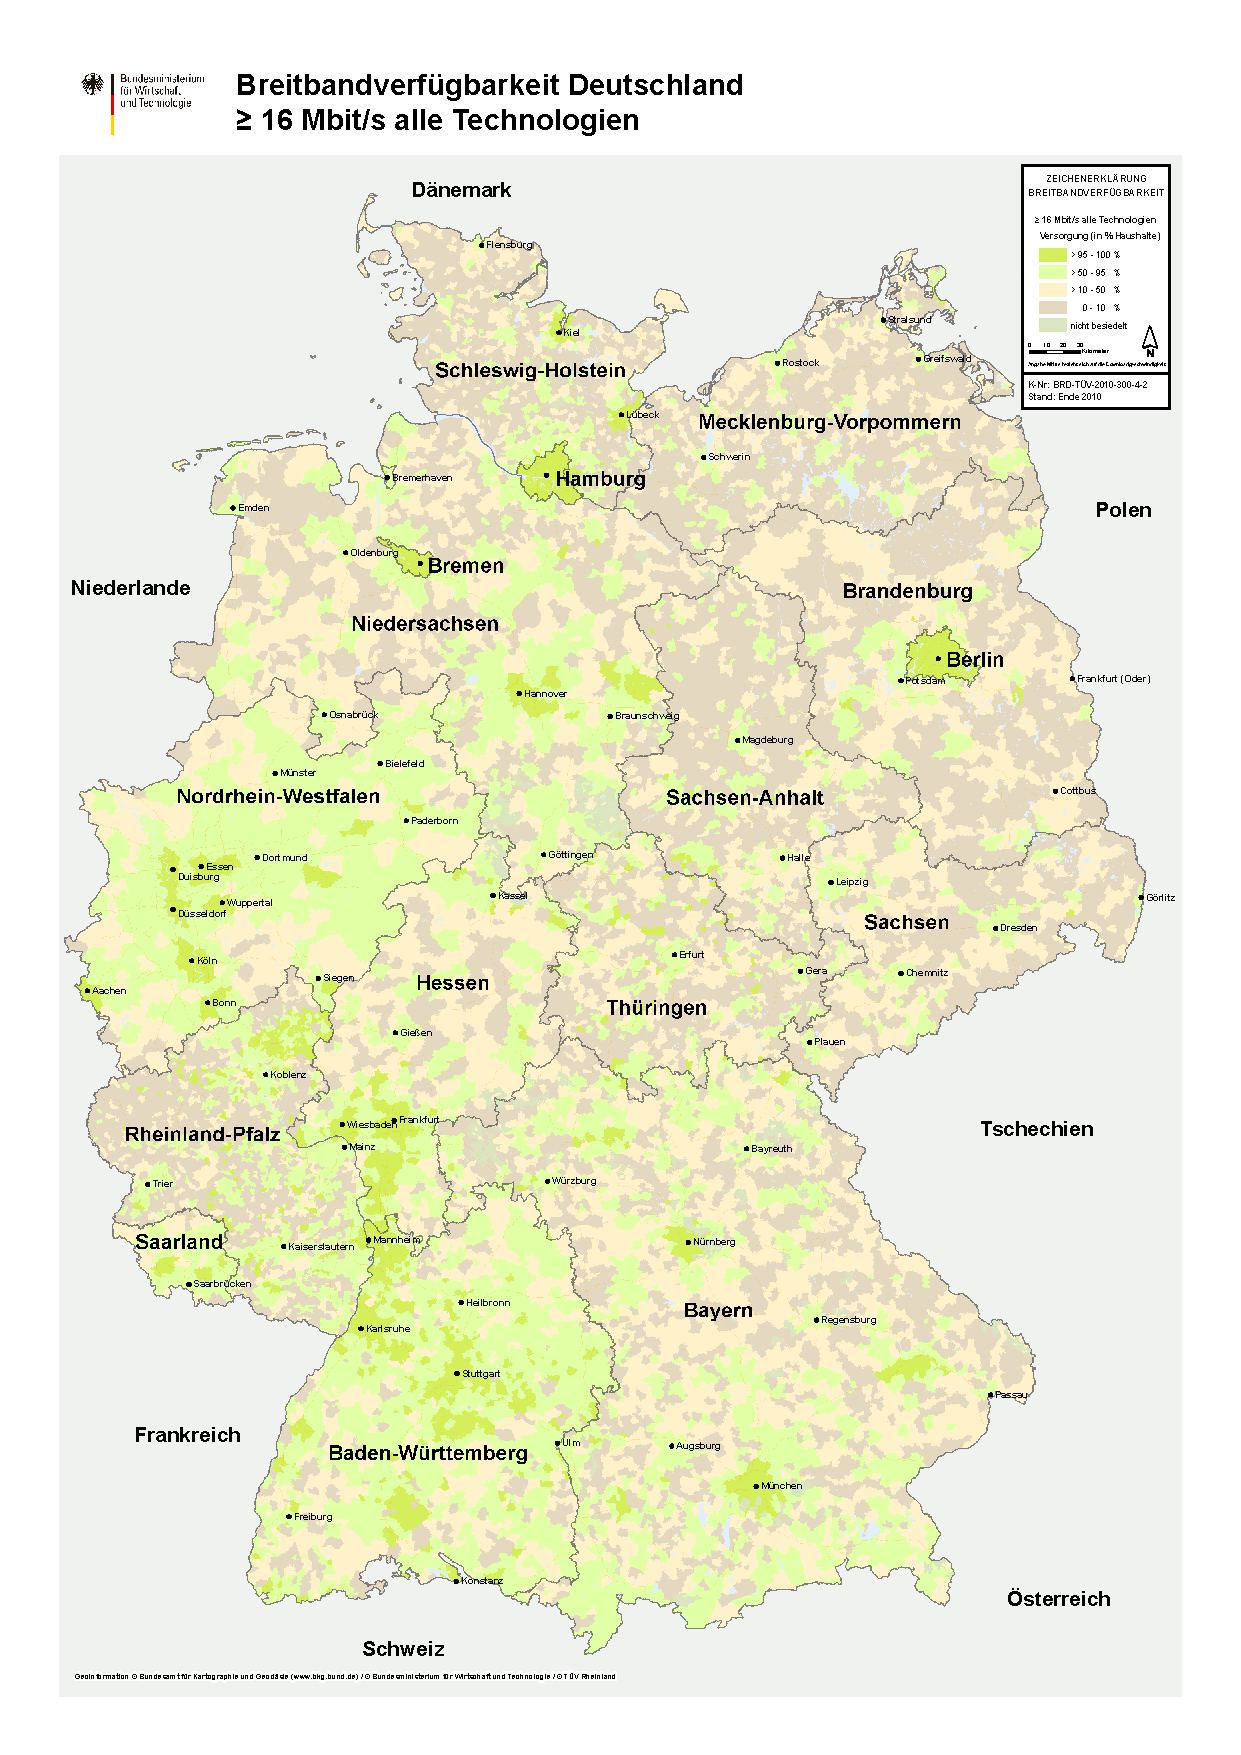
\includegraphics[scale=0.5]{material/breitband201116mbit.pdf}
  \caption{Breitbandversorgung mit 16Mbit/s oder mehr}
  \label{fig:breitband}
\end{figure}
In der Infografik in Abbildung \ref{fig:iwtfinfo}, die aus dem Internet World Stats Broadbrand Penetration Report der IWTF von 2009 abgeleitet wurde, sieht man Deutschland im Vergleich zu den führenden Industrienationen.\citep{Frucci2009} Der Unterschied zu unserem Nachbarland Frankreich ist sehr deutlich zu erkennen. Deutschland liegt auf dem 14. Platz mit ca 5Mbit/s und hat daher einen hohen Aufholbedarf.
\begin{figure}[!ht]
  \centering
  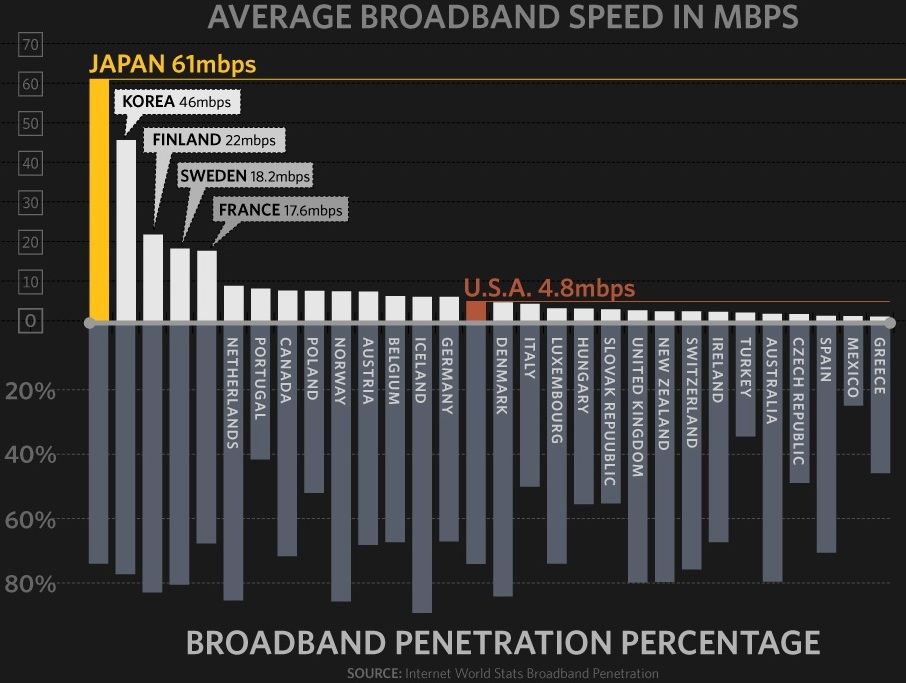
\includegraphics[scale=0.5]{material/worldinternetcomp.jpg}
  \caption{Ausschnitt aus einer Infografik des Internet World Stats Broadbrand Penetration Report der IWTF von 2009 }
  \label{fig:iwtfinfo}
\end{figure}
Um zu verdeutlichen, wie entscheidend die Geschwindigkeit des Internetzugangs für die Ladezeiten einer Webseite ist, folgt ein erläuterndes Beispiel:
Die durchschnittliche Webseitengröße beträgt 320 kB, wie im Abschnitt Ausgangszustand im praktischen Teil erläutert wird. Die üblichsten Anschlussgeschwindigkeiten betragen 1Mbit/s, 2Mbit/s, 6Mbit/s, 16Mbit/s, 25Mbit/s und 50Mbit/s. In der Tabelle wird die Zeit verglichen, die für die Übertragung von 320 kB mit den jeweiligen Bandbreiten, benötigt wird.
\begin{center}
    \begin{longtable}{ l | l | l | l | l | l | l}
    \hline
    Mbit/s & 1 & 2 & 6 & 16 & 25 & 50 \\ \hline
    \hline
	s für 320 kB & 2,6 & 1,3 & 0,44 & 0,16 & 0,1 & 0,05 \\ \hline
    \end{longtable}
\end{center}
Wenn die Ergebnisse in Relation zu den üblichen Ladezeiten im einstelligen Sekundenbereich gebracht werden, wird deutlich, wie groß der Einfluss der Bandbreite im ungünstigsten Fall werden kann.
\subsubsection{Browser}
Als Schnittstelle zwischen Nutzer und Webseite ist der Browser ein besonders kritischer Punkt und muss bei Web-Performanceanalysen besonders beachtet werden. Die meistgenutzten Browser sind der Internet Explorer, Mozilla Firefox, Google Chrome, Opera und Safari. In der Statistik in Abbildung \ref{fig:browseranteil} wird deutlich, dass der Internet Explorer, trotz der oft schlechteren Leistung, Marktführer ist.\citep{StatCounter2011}
\begin{figure}[!ht]
  \centering
  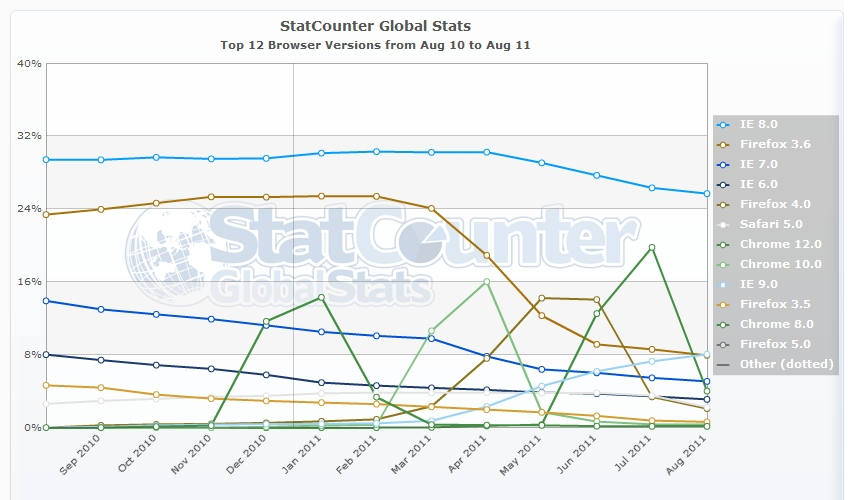
\includegraphics[scale=0.5]{material/browseranteil.jpg}
  \caption{Marktanteile der Browser von August 2010 bis August 2011 }
  \label{fig:browseranteil}
\end{figure}
Für Entwickler bedeutet die Browser-Vielfalt zusätzlichen Entwicklungsaufwand. Unrühmlichstes Beispiel ist der Internet Explorer 6.\footnote{Auszug aus Bugs des Internet Explorer 6: \url{http://www.dosonaro.com/6-der-haeufigsten-ie-bugs-und-wie-man-sie-behebt/}} Seine Kompatibilitätsprobleme sind so schwerwiegend, dass mittlerweile auch vom Hersteller Microsoft ein Update dringendst empfohlen wird.\footnote{Internet Explorer 6 Countdown: \url{http://www.ie6countdown.com/}}\citep{Microsoft2011} Um die Standardkompatibilität zu messen, wurden die Acid\footnote{\url{http://www.acidtests.org/}} Tests entwickelt. Der Internet Explorer 6 schafft im Acid3\footnote{Acid3 Test:\url{http://acid3.acidtests.org/}}-Test nur 11 von 100 Punkten. Moderne Browser, wie Google Chrome und auch der Internet Explorer 9, schaffen Werte über 90 von 100 Punkten. Neben Kompatibilität haben noch andere Leistungsparameter Einfluss auf die Ladezeiten. Die Javascript Ausführungszeiten kann man unter anderem mit dem SunSpider JavaScript Benchmark\footnote{Der Test wird direkt unter folgender URL angeboten: \url{http://www.webkit.org/perf/sunspider/sunspider.html}} testen. Einen Vergleich aktueller Browser zeigt Abbildung \ref{fig:sunspider}. Es wird deutlich, dass die Browser-Hersteller versuchen ein einheitlich gutes Level zu erreichen.  
\begin{figure}[!ht]
  \centering
  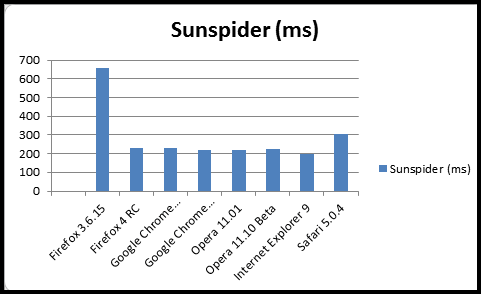
\includegraphics[width=0.9\textwidth]{material/sunspiderbenchmark.png}
  \caption{SunSpider Benchmark der letzten Browsergeneration}
  \label{fig:sunspider}
\end{figure}
Ein weiterer limitierender Faktor ist die künstliche Beschränkung der parallelen HTTP Zugriffe durch den HTTP/1.1 Standard. In diesem Standard wird unter anderem festgehalten, dass ein Client die Anzahl paralleler Verbindungen auf zwei beschränken soll. \citep{Fielding1999}
Das bedeutet, dass mehr Overhead zwischen den Übertragungen entsteht und die Inhalte nicht komplett parallel heruntergeladen werden k\"onnen. Diese Beschränkungen wurden eingeführt, da die Prozessorlast mit der Anzahl der Verbindungen zunimmt. Außerdem benötigen die Server mehr Arbeitsspeicher, wenn sie zusätzliche Verbindungen aufbauen. Aus Gr\"unden der Performance haben sich in den letzten Jahren die Browserhersteller von dieser Vorgabe entfernt. Aktuelle Browser ermöglichen sechs bis acht parallele Verbindungen, um die Bandbreite der Nutzer auslasten zu können. 
Zus\"atzliche Differenzen entstehen bei der DOM-Verarbeitung im Browser. Die Anzahl der enthaltenen Elemente steht grunds\"atzlich in negativer Korrelation zu der Geschwindigkeit mit der Operationen auf den Elementen durchgef\"uhrt werden k\"onnen. Ursache ist an dieser Stelle die Notwendigkeit, die Elemente zu selektieren und aufgrund dieser Tatsache muss \"uber alle Elemente iteriert werden. Die Zeit, die f\"ur diese Operationen ben\"otigt wird, steigt linear mit der Anzahl an Elementen.\citep{YahooDevNetwork2011}
Die verschiedenen Browser k\"onnen mit DOM-Elementen verschieden gut umgehen. \"Ahnlich wie bei der Javascript-Performance n\"ahern sich die neueren Browser-Generationen einander an.

\subsection{Serverseitige Probleme}
Moderne, dynamische Webanwendungen sind komplexe Applikationen. In vielen verschiedenen Bereichen kann es zu Problemen kommen. Nicht immer wirken sich diese direkt auf die Web-Performance beim Endnutzer aus. Oftmals werden einfach mehr Ressourcen als n\"otig genutzt. Dies resultiert aus mangelhafter Konfiguration oder Programmierung. 

\subsubsection{Netzwerkverbindung}
Wie auch beim Client spielt die Netzwerkverbindung des Servers eine entscheidende Rolle. Neben der beim Client erl\"auterten Latenz tritt beim Server die Bandbreite in den Vordergrund. Die Bandbreite ist das physische Limit an Auslieferungskapazität. Je gr\"o\ss{}er die Webseite ist, die ausgeliefert wird, desto weniger dieser Anfragen kann der Server befriedigen. Nat\"urlich unter der Bedingung, dass der Server in der Lage ist, die entsprechende Menge an Daten bereitzustellen. Wenn die auszuliefernden Daten statischer Natur sind oder es sich um gecachte dynamische Inhalte handelt, ist diese Menge normalerweise ausreichend, um die Netzwerkverbindung zu s\"attigen. 

%TODO tabelle basteln 
%100 kB/s * 1000 = 100 MB/s
%100Mbit/8 = 12 MB/s
  

\subsubsection{Datenbankabfragen}
So gut wie jede Webseite nutzt mittlerweile Datenbanken zur Verwaltung ihrer Datenbestände.
Oft sind diese Datenbanken ein Schwachpunkt für die Web-Performance, da meistens Daten von der Festplatte gelesen werden müssen und komplexe Abfragen viel Zeit in Anspruch nehmen können. Bei Applikationen, die mehreren Nutzern parallel Zugriff erm\"oglichen m\"ussen, kann es zu Problemen kommen, wenn die Datenbank Table-Locking verwendet. Dann wird die komplette Tabelle f\"ur Schreibzugriffe gesperrt, sobald ein Nutzer einen Datensatz manipuliert. Wenn solche F\"alle oft auftreten, sollte zum Row-Locking gegriffen werden, welches nur zeilenweise den Zugriff sperrt. Weitere Verbesserungen k\"onnen durch die geschickte Nutzung von Indizes erreicht werden. Indizes erreichen eine Beschleunigung von Abfragen die auf Spalten mit gro\ss{}en Feldgr\"o\ss{}en zugreifen. 

%\subsubsection{Skriptausführung}
%\subsubsection{Kompilierung}

\section{Wirtschaftliche Aspekte}
Web-Performance ist sehr wichtig f\"ur den wirtschaftlichen Erfolg von Projekten, die haupts\"achlich durch ihre Webseite repr\"asentiert werden.
\subsection{Usability}
Web-Performance hat einen großen Einfluss auf die Bedienbarkeit von Webseiten. Ohne die Innovationen im Gebiet der Web-Performance hätte Google mit GMail und ihren anderen Web-Applikationen keinen Erfolg erzielen können. Die Nutzer waren Desktop-Applikationen gew\"ohnt. Nur wenn eine Anwendung auch in einer akzeptablen Geschwindigkeit auf Benutzerinteraktionen reagieren kann, hat sie eine Chance auf dem Markt zu bestehen. Es gibt einige Studien, die sich mit Web-Usability auseinandersetzen. Zu den Ergebnissen gehörte unter anderem, dass langsamere Webseiten zu Vertrauensverlust sowie Nutzerfrustration führen. Als weitere Konsequenz ist der empfundene Qualitätsverlust zu nennen. Die genannten Punkte führen letztendlich zu niedrigeren Konversionsraten, das heißt, dass weniger Besucher zu Kunden werden. Zus\"atzlich steigt die Bail-out-Rate, welche beschreibt, wie viele Nutzer die Webseite w\"ahrend des Ladevorganges wieder verlasssen.\citep{Toll2011}

\subsection{Google Ranking}
Für (Internet-)Firmen ist es von immenser Bedeutung auf den vorderen Pl\"atzen der Google-Suche zu erscheinen. Ein Großteil der Internetnutzer sucht Angebote über die Google-Suche.\citep{Hitwise2011}
Google hat mit ihrer Initiative "`Let's make the web faster"'\footnote{\url{http://code.google.com/intl/de/speed/}} für viel Entwicklung und Aktivität im Bereich Web-Performance gesorgt und arbeitet zielgerichtet weiter in diese Richtung.\citep{Google2011} Dazu gehören seit 2008 Google AdWords\citep{AdWords2008} und seit 2010 die Google-Suche selbst. Dies stellt viele Unternehmen vor die Aufgabe, ihre Webseite zu optimieren und zu beschleunigen, um im Google-Ranking konkurrenzfähig zu bleiben. Wie genau Google die Webseiten testet, ist nur zum Teil bekannt, da diese Informationen zu Googles Geschäftsgeheimnissen gehören. Es finden sich aber einige Fakten, die bei der Optimierung für die Google-Suche, im Bereich Web-Performance, helfen können.
Bekannt ist, dass der Google-Suchmaschinen-Bot nichts mit der Geschwindigkeitsmessung zu tun hat und Google nur Daten von echten Nutzern, die die Google-Toolbar in ihrem Browser installiert haben, nutzt. Leider sind Daten nur für Internet Explorer ab Version 6 und Firefox ab Version 2 verfügbar. Als Kriterium für die Bewertung wird die Onload-Zeit gemessen. Dabei führt das verzögerte Nachladen von Inhalten zu einem besseren Ergebnis. Wenn eine Webseite für Google optimiert werden soll, muss also auch die Performance mit berücksichtigt werden. Performance ist aber nur ein Teil des Google-Rankings. Für Webseitenbetreiber gilt daher, dass aktuelle und gut strukturierte Inhalte nicht hinter die Performance gestellt werden dürfen.\citep{Bixby2011}

\subsection{Serverlast}
Eine umfassende Verbesserung der Auslieferungszeiten von Webseiten hat direkten Einfluss auf die Serverperformance. Dies ist leicht in einem Experiment feststellbar, wie folgende Überlegung zeigt: Wenn eine Webseite nur noch die Hälfte der Zeit benötigt, um ausgeliefert zu werden, hat man doppelt soviel Auslieferungskapazität zur Verfügung. Damit k\"onnen Kosten für Server und Traffic verringert werden. Außerdem ermöglichen Caching und Optimierungen einen Großteil an Prozessorlast einzusparen, der dann für andere Aufgaben zur Verfügung steht. Besonders wichtig ist die Performance in Momenten hoher Zugriffszahlen, beispielsweise wenn eine Webseite in einem prominenten News-Portal erwähnt wird. Oftmals bricht dann die Webseite zusammen, weil die Administratoren nicht mit solch einem Ansturm gerechnet haben. Erwähnenswert ist das Newsportal www.heise.de auf dem regelmäßig davon gesprochen wird, es wurde eine Webseite "`geheist"'\footnote{Eine Webseite wurde durch die hohe Anzahl der Zugriffe von Heise-Lesern \"uberlastet.}. Noch problematischer wird es, wenn ein Unternehmen Ziel krimineller Aktivitäten wird. Aktuell zu beobachten ist dieses Phänomen bei den Angriffen des Miner-Botnetzes auf mehrere deutsche Webseiten.\citep{Kaspersky2011} Um sich vor solchen Distributed Denial of Service (DDoS) Angriffen schützen zu können, ist eine performante Webseite sehr wichtig, um genug Ressourcen für Firewalls und andere Gegenmaßnahmen zur Verfügung zu haben. Gerade als kleine oder mittelgro\ss{}e Onlinefirma sollte man sich \"uber die Bedrohungen durch Erpresser im Klaren sein.


